\section{Problema 1: Laberinto}
\subsection{Introducción}

El escenario del primer problema es sencillo: dada una posición de arranque en un laberinto, queremos encontrar el costo del camino mínimo hacia una posición final. Para lograr esto podemos derribar hasta cierta cantidad, ya determinada, de paredes del laberinto mismo. El input total del problema consiste de:

    \begin{itemize}
        \item Una matriz $M$ de caracteres que representan el mapa, de dimensión $F\times C$ (pasados por parámetro) donde $M_{ij} \in \{$'$\cdotp$'$,$'$\#$'$,$'$o$'$,$'$x$'$\}$ según sea, respecto del orden listado del conjunto, un lugar caminable, pared, punto de origen o punto de destino. Se asume que existe un único caracter $'o'$ y un único $'x'$ en todo el mapa.
        \item Un entero $P$ que representa la cantidad máxima de paredes que podremos romper, es decir, caracteres $'\#'$ que pueden conformar el camino mínimo cuya longitud buscamos.
    \end{itemize}

También sabemos por enunciado que los caracteres del borde del mapa corresponden a una pared. Lo que quiere decir que $i \in \{0, F-1\} \ \vee \ j \in \{0, C-1\} \Rightarrow M_{ij} =\ $'$\#$'.

Teniendo en cuenta que cada movimiento realizado debe ser vertical u horizontal (los vecinos de $M_{i,j}$ son los elementos en rango del conjunto $\{M_{i+1,j},\ M_{i-1,j},\ M_{i,j+1},\ M_{i,j-1}\}$), podemos considerar el output del problema como la mínima longitud de las secuencias válidas de vecinos en el mapa, empezando por el punto de origen (sin contarlo, dado que no es una ubicación a recorrer, sino que es la primer ubicación 'recorrida' del mapa) y terminando en el punto de destino, con cantidad de caracteres $'\#'$ menor o igual a $P$. La idea se formaliza como:
\\

    \begin{itemize}
        \item $ M_{ij} = $'$ o $'$ $
        \item $A = \Big\{ \langle {M_{i_0, j_0}\ ...\ M_{i_{k-1}, j_{k-1}}} \rangle \ \Big | \kern 0.2cm
        M_{i_0,j_0} \in \{M_{i+1,j}\ M_{i-1,j}\ M_{i,j+1}\ M_{i,j-1}\} \kern 0.3cm \wedge \kern 0.3cm \sum\limits_{x=0}^{k-1} \beta(M_{i_x j_x} = $'$\#$'$) \leq P \kern 0.2cm \wedge \kern 0.2cm
        M_{i_{k-1}, j_{k-1}} = $'$\times$'$ \kern 0.3cm \wedge \kern 0.3cm
        \forall\ x \in [0..k-1) \kern 0.3cm M_{i_{(x+1)},j_{(x+1)}} \in \{M_{i_x+1,j_x}\ M_{i_x-1,j_x}\ M_{i_x,j_x+1}\ M_{i_x,j_x-1}\} \bigcap \\ M_{[1..F]\times[1..C]} \Big\}$
        \item $Output = \min\limits_{C \in A}\ |C|$
    \end{itemize}

Por ejemplo, sean los siguientes valores para $M$ y $P$:
\\
    \begin{center}
        $P=0, \kern 1cm
        M =
        \begin{bmatrix}
            \# & \# & \# & \# & \# \\
            \# & . & . & . & \# \\
            \# & \mathbf{o} & \# & \mathbf{x} & \# \\
            \# & . & . & . & \# \\
            \# & \# & \# & \# & \#
        \end{bmatrix}
        \kern 1cm
        (F = 5,\ C = 5)
        $

    \end{center}

Las secuencias de longitud mínima ($4$ en este caso) son los dos únicos caminos sin repetir ubicaciones: $\langle {M_{22}, M_{23}, M_{24}, M_{34}} \rangle$ y $\langle {M_{42}, M_{43}, M_{44}, M_{34}} \rangle$.

Para ilustrar un poco la idea del parámetro $P$ veamos también este caso:
\\
    \begin{center}
        $P=1, \kern 1cm
        M =
        \begin{bmatrix}
            \#  &   \#         &    \#    &   \#         &   \# & \#    \\
            \#  &   \mathbf{o}  &    \#     & \#          & \mathbf{x}    &   \#    \\
            \#  &   .         &    \#    &    .          &   .  & \#   \\
            \#  &   .          &    .     &   .          &   . & \#    \\
            \#  &   \#         &    \#    &   \#         &   \# & \#
        \end{bmatrix}
        \kern 1cm
        (F = 5,\ C = 6)
        $
    \end{center}

Si bien el camino más corto (obviando paredes) es $\langle {M_{23}, M_{24}, M_{25}} \rangle$, la suma de paredes atravesadas es $2 > P = 1$, por lo que tendremos que conformarnos la longitud $5$ del camino  $\langle {M_{32}, M_{33}, M_{34}, M_{35}, M_{25}} \rangle$
\\

El enunciado pide, además, una solución con complejidad $\mathcal{O}(FCP)$.

\subsection{Solución}

El enunciado pide abordar el problema desde una representación sobre grafos. Resulta bastante directo pensar cada nodo como el estado de nuestra ubicación en el mapa y cada arista como el movimiento hacia un vecino. Por lo tanto, nos interesa el camino en dicho grafo que menos aristas contenga.

Este tipo de problemas se puede resolver de manera generalizada con variaciones de $BFS$ (\emph{breadth-first search}), que nos aseguran recorrer el grafo por niveles de 'profundidad' (o sea, distancia de la raíz) y, por lo tanto, la primer solución que encontremos tendrá la misma o menor distancia al origen que cualquier otra. Esto se debe a que cada elemento se guarda en una estructura con organización \emph{'First In, First Out' (FIFO)}, y siempre estaremos visitando los estados del camino cuyo \emph{padre} haya sido visitado primero.

Nos queda ver cómo agregar las restricciones sobre la variable $P$ en esta representación. La idea de nuestra solución es ir guardando el estado de esta variable para cada camino armado y cortarlo cuando se supera la restricción.

En este pequeño ejemplo podemos ver tanto la idea de la representación en grafo del problema como del tipo de iteración que realiza $BFS$:

    \begin{center}
        $P=1, \kern 1cm
        M =
        \begin{bmatrix}
            \# & \# & \# & \# & \# \\
            \# & . & . & . & \# \\
            \# & \mathbf{o} & \# & \mathbf{x} & \# \\
            \# & \# & \# & . & \# \\
            \# & \# & \# & \# & \#
        \end{bmatrix}
        \kern 1cm
        (F = 5,\ C = 5)
        $

    \end{center}


    \begin{figure}[H]
        \centering
        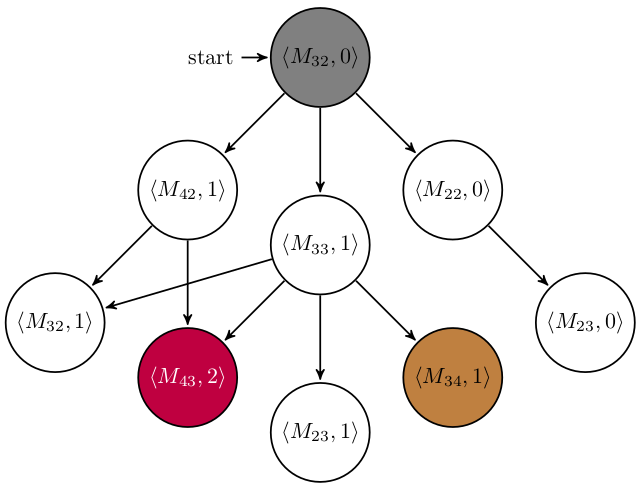
\includegraphics[width=12.0cm]{ej1-graph}
        \caption{El primer elemento de cada nodo revela la ubicación en el mapa y el segundo la cantidad de demoliciones contadas. El nodo rojo corresponde a un estado cuya rama, de seguir el algoritmo por no llegar ninguna rama al estado final en ese mismo nivel, sería podada. La longitud mínima de valor $2$ nos la da el camino $\langle {M_{33}, M_{34}} \rangle$}
        \label{fig:ej1-graph}
    \end{figure}

Una vez que, para algún nivel del grafo se llega a la posición final, el algoritmo termina y deja truncadas todas las demás ramas. Como veremos en el siguiente pseudocódigo, solamente vamos a agregar un estado cuando esa misma ubicación con esa misma cantidad de demoliciones no haya sido procesada anteriormente, de haberlo sido, entonces ya existe una manera de llegar al mismo nodo con menor o igual distancia al origen (porque lo vimos antes del actual). Esto hace que el algoritmo visite cada estado en forma arborea.

    \begin{lstlisting}

        dist[m][n][p+1] $\leftarrow$ (m $\times$ n $\times$ (p+1)) * (-1)
        cola<<y,x>, p> candidatos

        dist[origen.y][origen.x][0] $\leftarrow$ 0;
        candidatos.encolar(origen, 0);

        while $\neg$candidatos.vacio():
            cand $\leftarrow$ candidatos.desencolar()
            ubicacion $\leftarrow$ cand.first
            p_actual $\leftarrow$ cand.second
            distancia $\leftarrow$ dist[ubicacion.y][ubicacion.x][p_actual]

            if ubicacion = destino:
                return distancia

            $\textbf{para cada}$ vecino <x,y> de ubicacion que este en rango:
                p_vecino $\leftarrow$ p_actual + $\beta$(mapa[vecino.y][vecino.x] es pared)

                if p_vecino $\leq$ p_max $\wedge$ dist[vecino.y][vecino.x][p_vecino] $\neq$ -1:
                        candidatos.encolar(vecino, p_vecino)
                        dist[vecino.y][vecino.x][p_vecino] $\leftarrow$ distancia + 1
        return -1;

    \end{lstlisting}


\subsection{Complejidad}
